The catalogue screen initially retains 36 absorbers in 32 spectra. Extending the atmospheric exclusion to broad water bands leaves seven metadata candidates; actual-pixel inspection leaves six multiplet candidates. All six are retained in the physical-model accounting in Table~\ref{tab:archive_six}, including models that remain inadequate. These are selected DLA sightlines, not a complete or statistically representative sample of metal absorbers.

For the four newly modelled candidates, an exploratory adequacy gate requires $Q_0/(N-k_0)\leq1.5$, every line's $Q/N_{\rm line}\leq1.8$, and successful optimizer termination. The thresholds are working diagnostics under the stated diagonal errors, not calibrated goodness-of-fit probabilities. Component grids, windows and visible contamination warnings were recorded before the new relative-shift fits, with documented null-model grid extensions. Because an $H_0$ gate could also reject a genuinely shifted system, we additionally perform bounded free-shift and crossed-null diagnostics for both gate failures on their unchanged primary pixels. They remain inadequate, and we do not promote them to precision measurements or use the gate to infer population-level constancy.

\begin{table}[htbp]
\centering
\caption{Latest matched conventional/free-shift comparisons for all six archive candidates. $n_g$ is the shared gas-component count and $k_\delta$ the number of additional shifts. Values use native pixels and diagonal expected-fluctuation errors. ``Conditional'' permits a model-specific displacement diagnostic, not a calibrated atomic-frequency measurement. ``Inadequate'' retains the post-screen diagnostic comparison on the original primary data. All pairs retain model and optimization limitations described in the text.}
\label{tab:archive_six}
\small
\begingroup
\setlength{\tabcolsep}{4pt}
\begin{tabular}{lrrrrrl}
\toprule
Target ($z$) & Pixels & $n_g$ & $Q_0$ & $\Delta Q$ & $k_\delta$ & Status \\
\midrule
J232128$-$105122 (1.629) & 130 & 3 & 75.16 & 6.16 & 4 & Conditional \\
J225719$-$100104 (1.836) & 504 & 30 & 421.25 & 13.53 & 2 & Conditional \\
J053007$-$250329 (2.141) & 480 & 16 & 482.30 & 4.18 & 3 & Conditional \\
J233156$-$090802 (2.143) & 1176 & 26 & 1672.84 & 5.54 & 2 & Inadequate \\
J004131$-$493611 (2.248) & 138 & 6 & 95.23 & 7.97 & 2 & Conditional \\
J064326$-$504112 (2.659) & 436 & 16 & 532.23 & 4.64 & 3 & Inadequate \\
\bottomrule
\end{tabular}
\endgroup

\end{table}

The initial two pilots now have actual nuisance-refitted profiles for $D=v_{2382}-v_{2374}$ (Fig.~\ref{fig:archive_pair}). For J232128$-$105122, the latest matched full-model comparison gives $Q_0=75.1589$, $Q_1=68.9988$ and $\Delta Q=6.1600$ for four added shifts. Its $D=-339.97\,\mathrm{m\,s^{-1}}$ has unconstrained local tangent error $179.58\,\mathrm{m\,s^{-1}}$; the connected profile has linearly interpolated $\Delta Q=1$ crossings between optimized grid points at $[-495.18,-187.88]\,\mathrm{m\,s^{-1}}$. Several zero-level parameters are bound-active. Neither the local error nor the profile contour includes calibration or gas-architecture uncertainty.

J004131$-$493611 illustrates why a stopped optimizer is not a certified solution. Profiling discovered a substantially lower nuisance basin than the earlier pair $(Q_0,Q_1)=(110.0357,104.5341)$. Restarting both full hypotheses fairly gives $(95.2285,87.2549)$, hence $\Delta Q=7.9735$ for two shifts. The revised $D=-120.11\,\mathrm{m\,s^{-1}}$ has local tangent error $399.41\,\mathrm{m\,s^{-1}}$, whereas the bounded connected $\Delta Q=1$ contour, linearly interpolated between optimized grid points, is $[-264.86,+39.96]\,\mathrm{m\,s^{-1}}$. Active gas-width, response-width and zero-level bounds may contribute to this discrepancy; nonlinearity and residual curvature have not been separately isolated. These are conditional objective contours, not coverage-calibrated confidence intervals. Fixing $D=0$ still lets 1608 move and therefore does not recover the full $H_0$.

\begin{figure}[htbp]
\centering
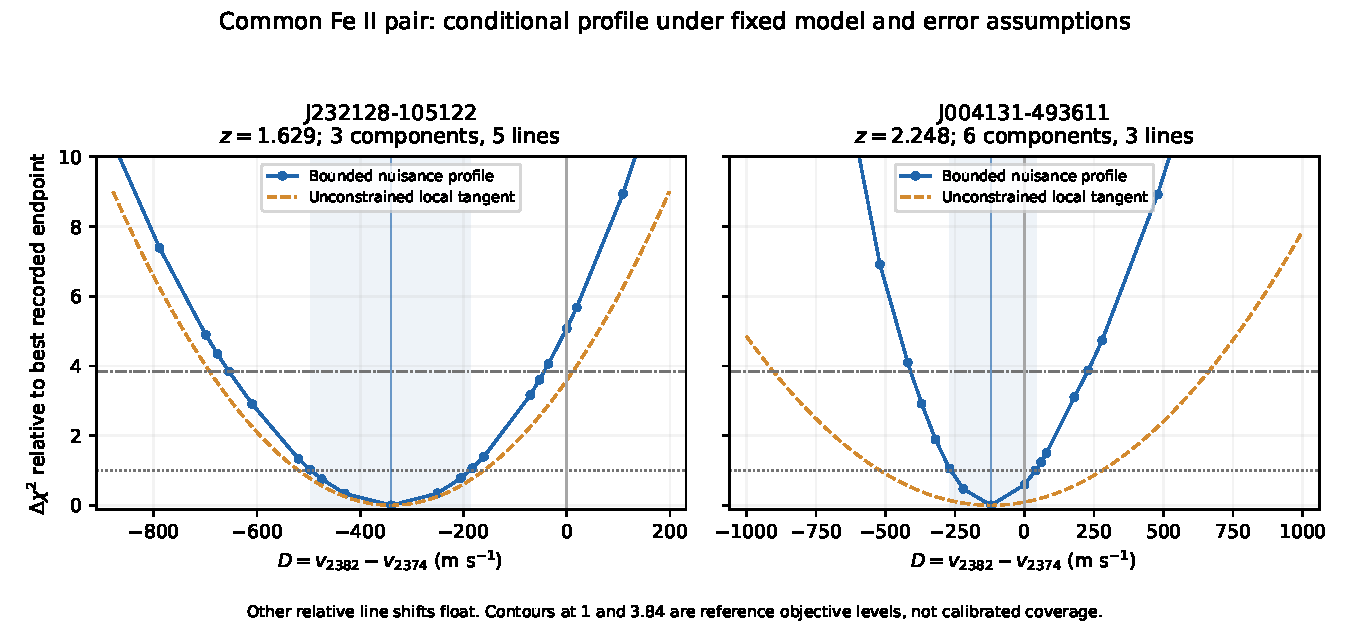
\includegraphics[width=.95\textwidth]{../experiments/highz_feasibility_2026-09-20/results/common_pair/common_pair_profiles.pdf}
\caption{Actual conditional profiles of the common 2382/2374 descriptor in the two initial pilots. Gas and other nuisance parameters, including the other relative line shifts, are refitted. Only endpoints in the final selected nuisance basins are connected; earlier inferior endpoints remain in the archive. Horizontal objective levels are descriptive. They do not calibrate systematic uncertainties, component selection or disconnected minima.}
\label{fig:archive_pair}
\end{figure}

The selected tested architecture for J053007$-$250329 has 16 gas components for four regions, including weak 1611, with 480 unique pixels. The matched comparison gives $\Delta Q=4.1760$ for three shifts. At this fixed architecture, $D=+268.78\pm130.09\,\mathrm{m\,s^{-1}}$ is a local conditional diagnostic; sparse nuisance-refitted offsets agree approximately with its local curvature. The count reaches the declared grid ceiling, two zero levels are bound-active, and 2374 retains structured residuals. Passing the working gate therefore does not establish model uniqueness or a frequency change.

For J225719$-$100104, the documented null-model grid extension reaches 30 components on 504 pixels. An audit retained a capped null endpoint with lower $Q$ than the initially selected successful endpoint; continuation and matched cross-starts then gave $Q_0=421.2482$ and $Q_1=407.7169$, an improvement of $13.5313$ for two shifts. This retains a conditional free-shift preference. The common descriptor is nevertheless $D=-15.74\pm228.84\,\mathrm{m\,s^{-1}}$ in the local tangent calculation, while 2344 lies at approximately $-355.68\,\mathrm{m\,s^{-1}}$ relative to 2374. Improvement of a multi-line model does not require a nonzero value of the particular common descriptor. A sparse five-point nuisance profile is asymmetric and its uppermost point reaches the evaluation cap; we do not present it as a completed calibrated interval. The bound-active gas width, finite component grid and first-order residuals remain limitations despite objective-based termination of the selected pair.


J064326$-$504112 retains all four primary lines and 436 pixels. Its 1611 window has a recorded sky-line warning and fails the per-line gate. Adding three shifts improves $Q$ by 4.6376 but leaves the 1611 objective per pixel at 2.0315. A separately labelled null-only omission control cannot replace the primary measurement. J233156$-$090802 uses a broad $[-480,+500]\,\mathrm{km\,s^{-1}}$ window, 26 components and 1176 unique pixels in three regions. Neighbouring 1611 opacity overlaps the red side of 1608 and is added before exponentiation; it is not counted as a second independent region on the same pixels. Two shifts improve $Q$ by 5.5433, but $Q_1/(N-k_1)=1.5381$ and the 2382 objective per pixel is 1.9036. The tested shifts do not resolve either target's main residual inadequacy. No precision $D$ interval is assigned to these systems.

The resulting inventory is richer than a catalogue of available spectra, but it is not six calibrated atomic measurements. Comparisons involve different component counts and line information, and successful objective-based stopping does not imply negligible first-order residuals or global optimization. Historical, unsuccessful and lower discovered endpoints are all preserved. We therefore use the six redshifts for the fixed-design calculations below, without fitting a physical age amplitude to these conditional offsets.
